\documentclass[12pt]{article}
\textwidth 15.5cm \oddsidemargin 0cm \topmargin -1cm \textheight
24cm \footskip 1.5cm \usepackage{epsfig}
\usepackage{amsmath,graphicx,psfrag,pstcol,pgfplots,tikz,filecontents,caption,listings,verbatim}
\def\n{\noindent}
\def\u{\underline}
\def\hs{\hspace}
\newcommand{\thrfor}{.^{\displaystyle .} .}
\newcommand{\bvec}[1]{{\bf #1}}
\pagestyle{plain}
%\pagenumbering{roman}
\begin{document}
\noindent
\vspace{3.6cm}
\begin{center}
{\bf ENGINEERING TRIPOS PART IIA\\\hfill \\
EIETL \\\hfill \\MODULE EXPERIMENT 3F3}
\end{center}
\vspace{0.5cm}
\begin{center}
{\bf RANDOM VARIABLES and RANDOM NUMBER GENERATION\\\hfill\\ H. Zhou \\\hfill\\
Jesus College \\\hfill
\\
hz324
}
\end{center}
\vspace{1.6cm}
\begin{center}
%
\includegraphics[width=3.6cm, keepaspectratio]{cam-logo-1.png}
\end{center}
\pagebreak
\section{\bf Uniform and normal random variables.}

{\bf Histogram of Gaussian random numbers overlaid on exact Gaussian curve (scaled):}\\
\begin{center}
    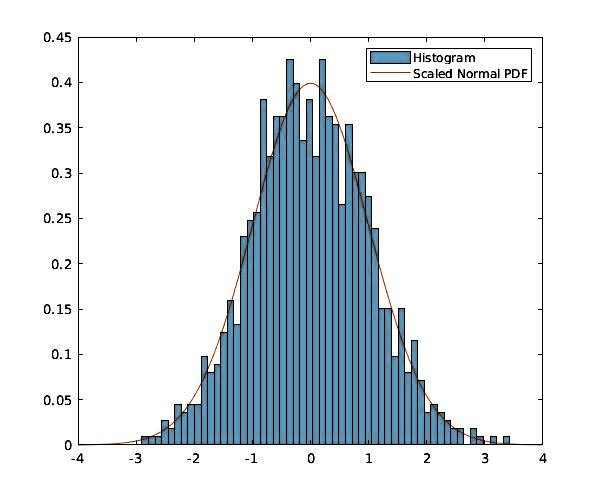
\includegraphics[width=0.666\textwidth]{norm-hist-1000.jpg}
    \captionof{figure}{\small\em Histogram of Gaussian random numbers on exact Gaussian curve (scaled)}
\end{center}
\\
{\bf Histogram of Uniform random numbers overlaid on exact Uniform curve (scaled):}\\
\begin{center}
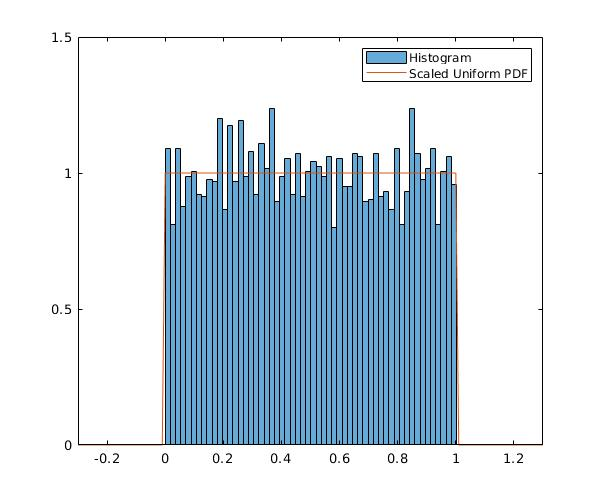
\includegraphics[width=0.666\textwidth]{uniform-hist-1000.jpg}
    \captionof{figure}{\small\em Histogram of Uniform random numbers on exact Uniform curve (scaled)}
\end{center}
\pagebreak
{\bf Kernel density estimate for Gaussian random numbers overlaid on exact Gaussian curve:}
\begin{center}
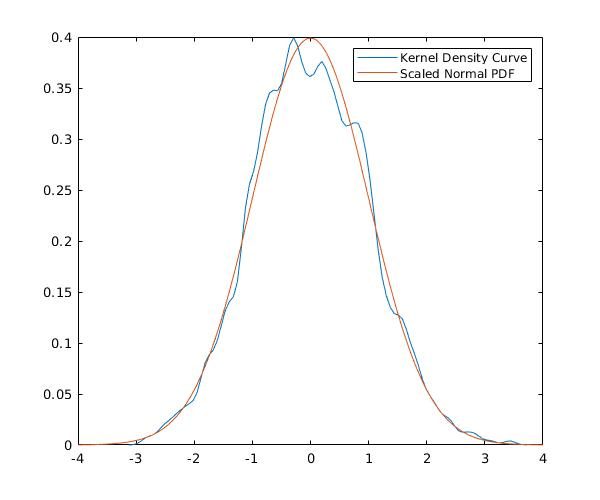
\includegraphics[width=0.6\textwidth]{norm-ks-1000.jpg}
    \captionof{figure}{\small\em Kernel density estimate for Gaussian random numbers exact Gaussian curve}
\end{center}
{\bf Kernel density estimate for Uniform random numbers overlaid on exact Uniform curve:}
\begin{center}
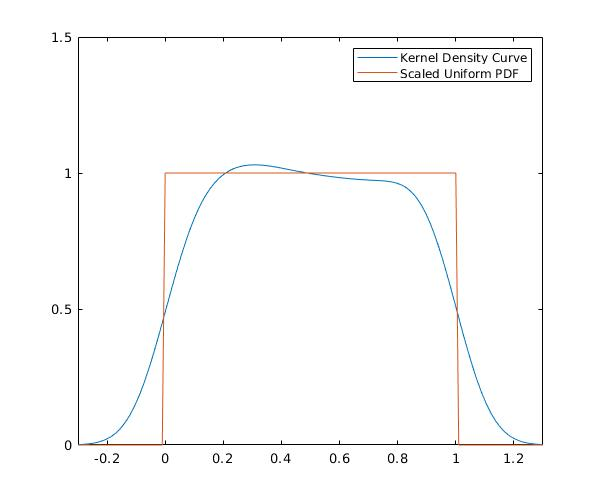
\includegraphics[width=0.6\textwidth]{uniform-ks-1000.jpg}
    \captionof{figure}{\small\em Kernel density estimate for Uniform random numbers  on exact Uniform curve}
\end{center}
\\
\pagebreak
{\bf Comment on the advantages and disadvantages of the kernel density method compared with the histogram method for estimation of a probability density from random samples:}
\\\\
{\small\textsf
The histogram has a few advantages. It, first of all, requires relatively small amount of computing power, since the complexity of generating such histogram is ~$O(n)$. Only a linear search through the sample space seems to be needed.
\par\bigskip
More importantly, the histogram models a discontinuous step much better than a kernel density curve. The histogram represented the uniform distribution much better than the kernel density method.
\par\bigskip
The kernel density method, however, is able to model a continuous pdf much better than that of a histogram. We can see from the figures above, that the kernel density estimation gave a much better curve that fitted the gaussian PDF.
\par\bigskip
Despite it's advantage in continuous PDFs, the kernel density estimation seems to have a complexity of ~$O(n^2)$, each datapoint in the sample space needs to be computed taking into all other datapoints.
\par\bigskip
This estimation method also doesn't model a step very well. In the uniform distribution case, a very flat and unrealistic gradient was seen on both of the step of a uniform PDF.
\par\bigskip
}
\\
{\bf Theoretical  mean and standard deviation calculation for uniform density as a function of $N$:}
\\\\
{\small\textsf
From multinomial distribution theory, we get
\[\mu = Np_j \text{ and } \sigma = \sqrt{N(1-p_j)p_j},\text\]
where $p_j$is the probability of a sample lies in bin j.
In the uniform case, \[{math} p_j = 1/J \], where J is the total bin number.
\par\smallskip
Thus, the mean and standard variation are \[ \mu =  N/J \text{ and } \sigma = \sqrt{N(J-1)/J^2} \]
}
\\
{\bf Explain behaviour as $N$ becomes large:}
\\\\
{\small\textsf From the weak law of large numbers, the value of each bin should tend to the theoretical mean. In our case \[\lim_{N \to \infty} P(|X_i-\mu| \geq \epsilon) = 0\]
    Where $X_i$ is the number of random variable in each bin.
    \par\bigskip
    This means that the variation is a lot smaller with the histogram fitting the theorectical $\mu$ line in this case.
}\\
\par\bigskip
\pagebreak
\\
{\bf Plot of histograms for $N=100$,  $N=1000$ and $N=10000$ with theoretical mean  and $\pm 3$ standard deviation lines:}
\begin{center}
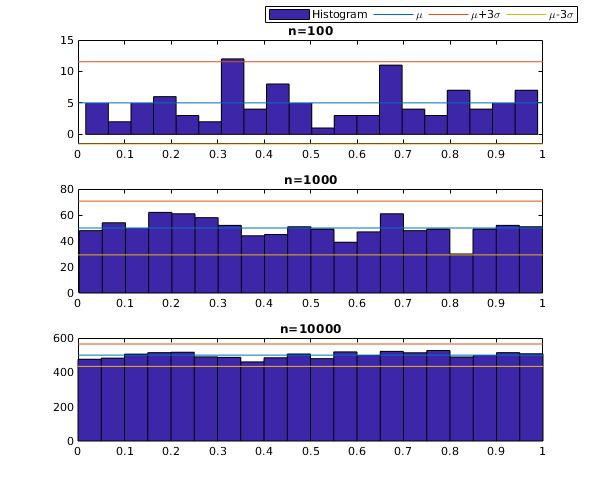
\includegraphics[width=0.81\textwidth]{uniform-n-fit.jpg}
    \captionof{figure}{\small Histograms for $N=100$,  $N=1000$ and $N=10000$ with theoretical mean  and $\pm 3$ standard deviation lines}
\end{center}
\\
{\bf Are your histogram results consistent with the multinomial distribution theory?}
\\\\
{\textsf
 All bins lied within the $\pm 3\sigma$ lines, hence it was indeed consistent with the theory.
}
\par\bigskip
\section{\bf Functions of random variables}\\
{\bf For normally distributed ${\cal N}(x|0,1)$ random variables, take $y=f(x)=ax+b$. Calculate $p(y)$ using the Jacobian formula:}
\\\\
{\em
\begin{equation*}
\begin{split}
  p(y)& = \left.\frac{p(x)}{|dy/dx|}\right|_{x=f^{-1}(y)} \\
      & = \left.\frac{N\left(x\middle|0,1\right)}{|a|}\right|_{x=\frac{y-b}{a}} \\
      & = \frac{1}{\sqrt{2\pi}|a|}\exp{(-\frac{(y-b)^2}{2a^2})}
\end{split}
\end{equation*}
}
\pagebreak
\\
{\bf Explain how this is linked to the general normal density with non-zero mean and non-unity variance:}
\par\smallskip
{\textsf
By inspection, the transformed random variable is a normal distribution with $\mu =b$ and $\sigma =|a|$.This can also be verified.
\par\smallskip
With the random variable as X
\[
E[aX+b] = aE[X] + b = b \\
Var[aX+b] = a^2Var[X] = a^2  
\]
This agrees with the previous Jacobian result.
}
\par\bigskip
\\
{\bf Verify this formula by transforming a large collection of random samples $x^{(i)}$ to give $y^{(i)}=f(x^{(i)})$, histogramming the resulting $y$ samples, and overlaying a plot of your formula calculated using the Jacobian:}
\\
\begin{center}
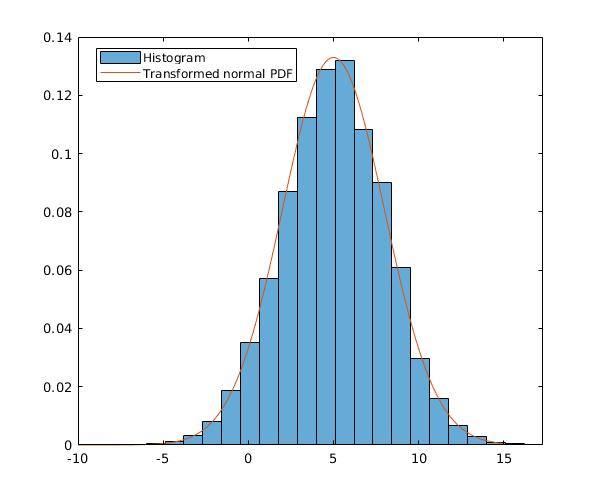
\includegraphics[width=0.9\textwidth]{norm-lin-y.jpg}
    \captionof{figure}{\small Linear transform on a gaussian variable}
\end{center}
\pagebreak
{\bf Now take $p(x)={\cal N}(x|0,1)$ and $f(x)=x^2$. Calculate $p(y)$ using the Jacobian formula:}
\par\bigskip
{\textsf The inverse $f^{-1}(y)$ does not have a unique solution this time, so we'll consider all cases:\\
\begin{equation*}
\begin{split}
  p(y) & = \sum_{k=1}^2{\left.\frac{p(x)}{|dy/dx|}\right|_{x=f^{-1}(y)}} \\
       & = \left.\frac{p(x)}{|2x|}\right|_{x=\sqrt{y}}+\left.\frac{p(x)}{|2x|}\right|_{x=-\sqrt{y}} \\
       & = \frac{p(\sqrt{y})}{|\sqrt{y}|}\\
       & = \frac{1}{\sqrt{2\pi y}}\exp{(-\frac{y}{2})}
\end{split}
\end{equation*}
}
\\
{\bf Verify your result by histogramming of transformed random samples:}
\\
\begin{figure}[h]
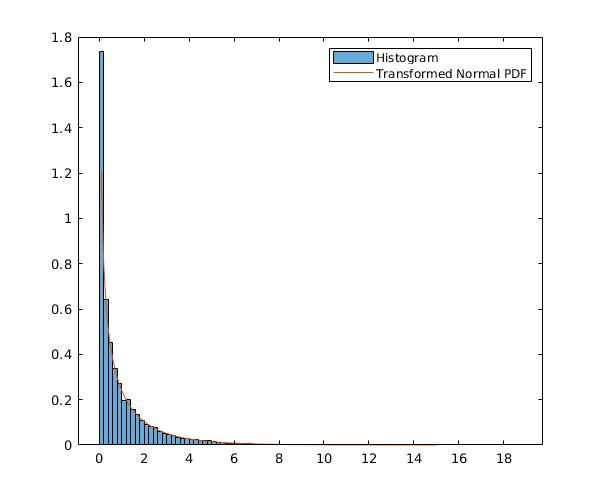
\includegraphics[width=0.9\textwidth]{norm-parabo-y.jpg}
  \caption{Quadratic transform on a gaussian variable}
  \label{fig:Quadratic transform on a gaussian variable}
\end{figure}\\
\pagebreak
\section{\bf Inverse CDF method} 



{\bf Calculate the CDF and the inverse CDF for the exponential distribution:}
\\
{\em
\begin{equation*}
\begin{split}
  x = F(y) & = \int_0^y \mathrm \exp{(-t)} \mathrm dt \\
           & = 1 - exp(-y) , y\geq0. \\
   exp(-y) & = 1-x \\
   y & = -ln(1-x) \quad (0 \leq x < 1)        
\end{split}    
\end{equation*}   
}
\\
{\bf Matlab code for inverse CDF method for generating samples from the exponential distribution:}
\begin{verbatim}
% Random variable generation with the calculated cdf:
% 10,000 number of samples
n=10000
% Generating uniform random variable
x1=rand(n,1);
%Convert uniform random variable to  the desired exponential random variable
y=-log(1-x1);
\end{verbatim}
\\
{\bf Plot histograms/ kernel density estimates and overlay them on the desired exponential density:}

\begin{center}
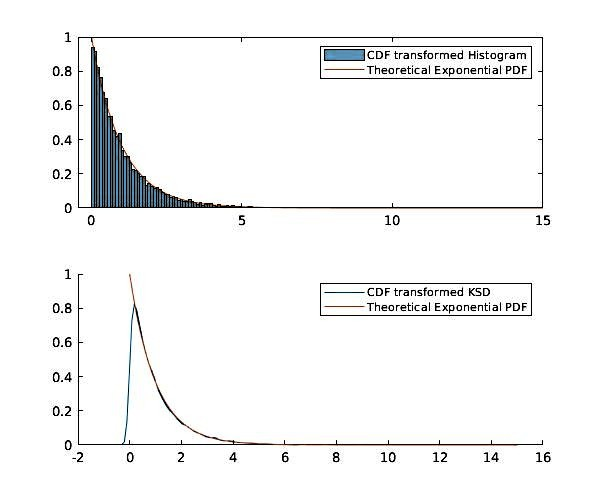
\includegraphics[width=0.81\textwidth]{cdf-method-exp.jpg}
    \captionof{figure}{\small Histograms/kernel density estimates on the desired exponential PDF}
\end{center}

\section{\bf Simulation from a `difficult'  density.}

{\bf Matlab code to generate $N$ random numbers drawn from the distribution of $X$:}
\\\\
\begin{lrbox}{\myv}\begin{minipage}{\textwidth}
\begin{verbatim}
% Random variable generation with the numerical 'recipe':
% 10,000 number of samples
n=10000;
% Initialising parameter alpha and beta
alpha = 0.5;
beta = 0.9;
% Evaluating b and s
b=(1/alpha)*atan(beta*tan(pi*alpha/2));
s=(1+beta^(2)*(tan(pi*alpha/2))^(2))^(1/(2*alpha));
% Sampling u and v from uniform and exponential PDFs respectively
u=(-pi/2) + rand(n,1)*pi;
v=exprnd(1,n,1);
% Generate x, random variable of interest, from the numerical 'recipe'
x = s*(sin(alpha*(u+b))./(cos(u)).^(1/alpha)).*(cos(u-alpha*(u+b))./v).^((1-alpha)/alpha);
\end{verbatim}
\end{minipage}\end{lrbox}
\resizebox{0.95\textwidth}{!}{\usebox\myv}
\\\\
{\bf Plot some histogram density estimates with $\alpha=0.5,\,1.5$ and several values of $\beta$:}
\begin{center}
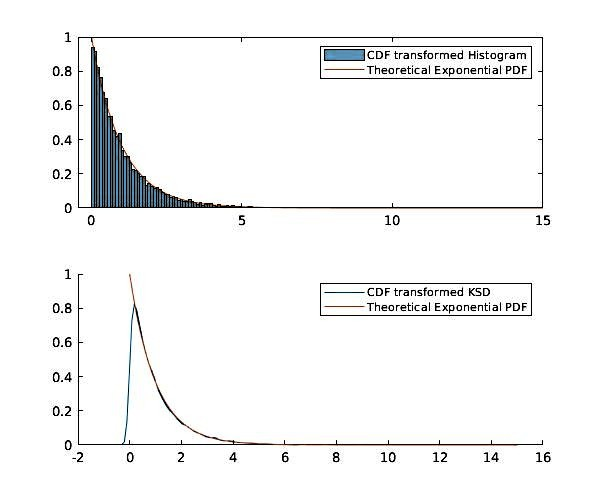
\includegraphics[width=0.9\textwidth]{cdf-method-exp.jpg}
\captionof{figure}{\small Histograms with various $\alpha$ and $\beta$ values}
\end{center}
\\
\pagebreak
{\bf Hence comment on the interpretation of the parameters $\alpha$ and $\beta\in[-1,+1]$:}
\\\\
{\textsf
Inferring from the plots, the parameter $\alpha$ changes the slope of the distribution. The curve becomes narrower and steeper as $alpha$ gets smaller. Hence this parameter $alpha$ can be, perhaps treated as a 'characteristic exponential term'.\\\\
The parameter $\beta$ however, seems to have effect on the skewness of the the curve. A characteristic skew term, if you will. When $\beta >0$, the curve is positive skewed and negatively skewed when $\beta <0$. The curve seems to symetrical  with no skewness at $\beta =0$
}
\end{document}


